% % % % % % % % % % % % % % % % % % % % % % % % % % % % % % % % % % % % 
% 
% FS-Vorlage											Stand: 30.01.12
%
% Formelsammlungsvorlage von Emanuel Regnath und Martin Zellner	
% Bietet verschiedene Abkürzungen und Befehle	
%
% % % % % % % % % % % % % % % % % % % % % % % % % % % % % % % % % % % % 


% Dokumenteinstellungen
% ======================================================================

% Dokumentklasse (Schriftgröße 6, DIN A4, Artikel)
\documentclass[fs, footer]{latex4ei}


% Dokumentbeginn
% ======================================================================
\begin{document}


% Aufteilung in Spalten
\begin{multicols*}{4}

\fstitle{Digitale Sprach- und Bildverarbeitung}
% -------------------------------------------
% | 		Regelungssysteme				|
% ~~~~~~~~~~~~~~~~~~~~~~~~~~~~~~~~~~~~~~~~~~~
\section{Grundlagen der Mustererkennung}
% ======================================================================

\textbf{Messung} $\ra$ Vorverarbeitung $\ra$ \textbf{Merkmalsextraktion} $\ra$ \textbf{Klassifikation}\\
\\
\subsection{Klassifikatoren}
Lernphase eines Klassifikators: Testsignale, Einstellen der Parameter.\\
Re-Klassifikation: Bereits bekannte Signale\\
Cross-Klassifikation: Neue Signale\\
\begin{description}
	\item[Nearest-Mean] Mittelsenkrechte zu beide Mittelwerten (2D)
	\item[$k$-Nearest-Neighbor:] Minimum des Abstand zu $k$ nächsten Nachbarn
\end{description}

\subsection{Erkennungsraten}
\begin{tabular}{lcc}
	& 1. Kl. ist & 2. Kl. ist\\
1. Kl. erkannt & \textcolor{teal}{A} & \textcolor{red}{B}\\
2. Kl. erkannt & \textcolor{red}{C} & \textcolor{teal}{D}\\
\end{tabular}\\
\\
Accuracy: $\frac{\text{Richtige Klassifikation}}{\text{Gesamtzahl}} = \frac{A+D}{A+B+C+D}$\\
Precision $\frac{\text{Richtige Klasse 1}}{\text{Erkannte Klasse 1}} = \frac{A}{A+B}$ \qquad „Ich sage A, ist es A?“\\
Recall $\frac{\text{Richtige Klasse 1}}{\text{Tatsächliche Klasse 1}} = \frac{A}{A+C}$\qquad „Es ist A, sage ich A?“\\
False Acceptance Rate (FAR): $\frac{\text{Falsch angenomme 1}}{\text{Alle 2}} = \frac{B}{B+D}$\\
False Rejection Rate (FRR): $\frac{\text{Falsch abgelehnte 1}}{\text{Alle 1}} = \frac{C}{A+C}$

Nich-Lineare Klassifikatoren: Polynom, Support-Vector-Machines, KNN


\section{Frequenzanalyse}
% ======================================================================

	\subsection{Diskrete Fouriertransformation}
	Frequenzauflösung: $\Delta f = \frac{f_{\ir s}}{N}$
	
	
	\subsection{Fensterung}
	Abtastwerte = Frequenz $\cdot$ Fensterdauer

	\subsection{Center-Clipping}
	Reduziert den Einfluss der ersten Formanten:\\
	$y(k) = \begin{cases} 1 & s(k) \ge C_L \\ 0 & \abs{s(k)} < C_L \\ -1 & s(k) \le -C_L \end{cases}$
	
	\subsection{Autokorrelationsfunktion AKF}
	Unempfindlich für Rauschen, Empfindlich für Formanten
	
	\subsection{Cepstrum}
	$\mathrm{CEP} = \mathrm{DFT}\{ \log \abs{S(n)}^2 \}$, Empfindlich für Rauschen
	
	\subsection{Spektrogramm $\abs{f(t,\omega)}$}
	Kurzzeitspektrum: Abschnitte (Fenster) werden als stationär betrachtet.
	Zeitlicher Verlauf des Leistungsspektrum. \\
	Zeitliche Auflösung $\propto^{-1}$ Frequenzauflösung
	


\section{Sprachanalyse}
% ======================================================================
	\begin{tabular}{ll}
	stimmhaft (Vokale / lange Konsonanten) & stimmlos (kurze Konsonanten)\\
	periodischer ZB & rauschähnlicher ZB\\
	große Amplituden & kleine Amplituden\\
	Maxima im FB & Zappeln bei hohen Freq.\\
	
	
	\end{tabular}
	

	\subsection{Stimmhaft}
	Erstes Maximum: Grundfrequenz\\
	Zweites Maximum: 1. Formante\\
	Drittes Maximum: 2. Formante\\

	Grundfrequenz bestimmen mit AKF: Bei Rauschen\\
	Grundfrequenz bestimmen mit Cepstrum: Bei starken Formanten\\



	\subsection{Lineare Prädiktion}
	Aus vorherigen Signalwerten den nächsten schätzen.\\
	Schätzwert $\hat s = \sum\limits_{i = 1}^p \alpha_i s(k-i)$\\
	\\
	Datenreduktion pro Fenster: $\frac{N - (p+3)}{N}$\\
	\\
	Durban Algorithmus ($\alpha_0 = -1$):\\
	$E^{(0)} = R(0)$\\
	$k_1 = \alpha_1^{(1)} = \frac{R(1)}{E(0)}$ \qquad Mittl. Quadr. Fehler $E^{(1)} = (1-k_1^2)E^{(0)}$ \\
	$k_2 = \alpha_2^{(2)} = \frac{R(2) - \alpha_1^{(1)} R(1)}{E^{(1)}}$\\
	$\alpha_1^{(2)} = \alpha_1^{(1)} - k_2 \alpha_1^{(1)}$\\
	Koeffizienten $\alpha_j = \alpha_j^{(p)}$


	\subsection{Merkmalsextraktion}
	soll den Umfang der in die Erkennung eingehenden Daten reduzieren.\\
	Redundant sind für der Spracherkennung alle sprecher- und situationsspezifischen
	Informationen, benötigt wird nur die Information darüber, \emph{welches} Wort gesprochen wurde.\\
	Ergebnis ist der Merkmalsvektor $\vec m_j$, für ein Fenster die Matrix $\ma M = \mat{\vec m_1 & \vec m_2 & ...}$
	
	\begin{description}
		\item[Frequenzbandkoeffizienten (FBK):] FT, LDS: Mittlere Signalleistung einzelner Intervalle
		\item[Melfrequenz-Cepstral-Koeff. (MFCK):] gehörrichtige Bewertung der Frequenzskala und gute Dekorrelation der Koeffizienten
		\item[Autokorrelationskoeffizienten (AKK):] AKF: $m_j = \frac{\overline{\text{AKF}}(j)}{\overline{\text{AKF}}(0)}$
	\end{description}


	\subsection{Mustervergleich}
	Muster $\ma M$, Referenzmuster $\ma R^{(k)}$
	\begin{enumerate}
		\item Ermittlung der Distanzmatrix $\ma D$
		\item Dynamic Time Warping (DTW)
		\item Backtracking
	\end{enumerate}



\section{Sprechererkennung}
% ======================================================================
\begin{description}
	\item[Sprecherverifikation:] Eine Identität anhand eines Musters verifizieren(prüfen)
	\item[Sprecheridentifikation:] Eine Identität in verschiedenen Muster erkennen(suchen)
\end{description}


	\subsection{Merkmalsgewinnung}
	\begin{enumerate}
		\item Aufnehmen mit $\SI{16}{\kilo \hertz}$ und $\SI{16}{bit}$
		\item Höhenanhebung, da Stimme Tiefpasscharakter
		\item FFT (Kurzzeitspektrum mit 256 Freq.) mit Hamming Fenster
		\item Merkmalsgewinnung: 
			\begin{enumerate}
				\item Pausen($E_{\min}$) entfernen, da Rauschen sonst charakteristisch werden
				\item Reduktion von 256 auf $K$ Frequenzkanäle $A_k$ ($K \approx [10,30]$)\\
					Mittelwert aus immer $R = \frac{K'}{K}$ folgenden
				\item Näherung des Langzeitspektrums: Amplituden Mittelwert für alle $n$ Zeiten: $x_k = \frac{1}{N} \sum A_k[n]$
			\end{enumerate}
		\item Speichern der normierten Merkmalsvektoren
	\end{enumerate}

	\subsection{Klassifikation}
	\begin{description}
		\item[Minimal-Abstands-Klassifikator(MinAK):] Eukl. Abstand der Testvek. $(\vec x^M - \vec x^R)^2 < \varepsilon$\\
		\item[Einzeltoleranz-Klassifikator(EK):] Einzelne Spektralwerte vergleichen. $\abs{x_i^M - x_i^R} < \varepsilon_i$\\
		\item[Mahalanobis-Abstands-Klassifikator(MahAK):] Berücksichtig Streuung zwischen Frequenzen durch viele Lernstichproben
	\end{description}





\section{Bildverarbeitung}
% ======================================================================
Speicherbedarf: $\text{Dim.}_x \cdot \text{Dim.}_y \cdot \text{Kanäle}_k \cdot \text{Tiefe}_m$\\
Anzahl Graustufen: $L = 2^m$\\
Zusammenhang: $N/2 \Ra 4m \Ra 16L$


	\subsection{Farbräume}
	\begin{tabular}{llll}
	RGB & Grundfarben (Rot, Grün Blau) & Bildschirmpixel\\
	CMY & Grundfarben (Cyan, Magenta, Yellow) & Druckerfarben\\
	YUV(YIQ) & Y = Luminaz , U und V = Chrominanz & Video(PAL)\\
	CIE & Farbebene x,y & Normtafel\\
	\end{tabular}
	
	Luminanznormierung: Helligkeitsinformationen auf ein Intervall zwischen $[0,1]$\\
	Histogramm: Säulendiagramm aller vorkommenden verschiedenen Intensitäten\\
	Grauwerttransformationen: Histogrammgleichung\\


	\subsection{Bilineare Interpolation}
	$x_{\Delta} = \frac{x_s}{\Delta x} - i$ \qquad $y_{\Delta} = \frac{y_s}{\Delta y} - j$\\
	$f_K(x_s, y_s) = (1-x_{\Delta})(1-y_{\Delta}) p_{i,j} + (1-x_{\Delta}) y_{\Delta} p_{i,j+1} + x_{\Delta} (1-y_{\Delta}) p_{i+1,j} + x_{\Delta} y_{\Delta} p_{i+1,j+1}$\\
	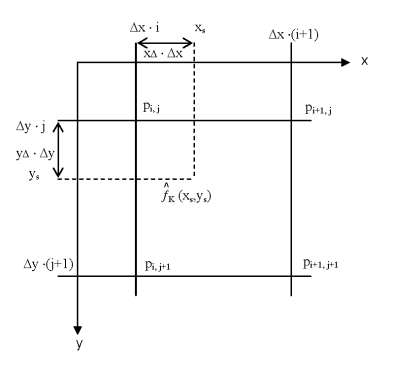
\includegraphics{./img/billinear.png}
	
	\subsection{JPEG Kompression}
	\begin{enumerate}
		\item Unterteilung in 8x8 Pixel-Blöcke, Symmetrisierung [0,255] $\ra$ [-127,128]
		\item Discrete Cosine Transformation (DCT): Ortsspektrum, Vor- und Rücktrafo symmetrisch
		\item Quantisierung: (Wert / Tabelle) abrunden: $Q(W/T) = \floor{W/T}$
		\item Entropiecodierung: \\
			Zick-Zack: Nullen am Ende durch “EOB” ersetzen\\
			Lauflängenkodierung, Huffmancode
	\end{enumerate}
	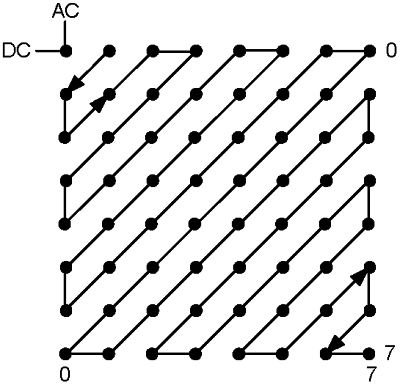
\includegraphics[width = 3cm]{./img/zickzack.png}


% Ende der Spalten
\end{multicols*}

% Dokumentende
% ======================================================================
\end{document}

% ToDos:

